\section{The joint electron--lattice response}\label{sec:12.1}

At a momentum transfer of \SI{50}{keV} a silicon nucleus receives the recoil energy $E_R = q^2/2M_\kappa = \SI{47.8}{meV}$. The lattice takes the recoil energy as a few phonons: the Debye--Waller exponent is $2W_\kappa = 1.57$, and in \SI{21}{\percent} of the kicks the lattice is left as it was (\cref{sec:11.3}). In about three kicks in a million, in the model of \cref{fig:12-plane} below, the electrons do not follow the nucleus, and an electron--hole pair of a few eV is made as well. An event with a pair deposits about \SI{6}{eV}, of which \SI{48.5}{meV} are in the lattice and the rest in the electrons, and a detector treats the two parts differently. The electronic energy makes charge at once; the lattice energy lies below the gap and reaches only a phonon sensor (\cref{chap:18,chap:20}). The response $S_{ab}(\vect{q},\omega)$ of the master formula \cref{eq:8.2-spectrum} cannot separate the electronic energy from the lattice energy, because it adds all final states of the same total energy $\omega$. We need a response with two energy arguments.

\subsection{The joint response}\label{sec:12.1-def}

Every prompt final state $f$ of \cref{sec:8.7-classes} has a definite electronic content: none in the electron-following sector, and otherwise an electron--hole pair, an exciton or a core hole, with or without phonons. We give it an \emph{electronic energy} $E^{\mathrm{el}}_f$, zero in $\mathcal{P}_{\mathrm{ad}}$ and otherwise the zero-phonon energy of its electronic excitation; for a pair this is the quasiparticle energy $\tilde E_m$ of \cref{eq:8.6-dyson}. The remaining energy of the final state, $E_f - E^{\mathrm{el}}_f$, belongs to the lattice: phonons and a recoil. Sorting the final-state-resolved response \cref{eq:8.7-resolved} by the two energies defines the \emph{joint response}
\begin{equation}
  S_{ab}(\vect{q};\omega_l,\omega_e) = \frac{2\pi}{\Vol}\sum_{i,f}p_i\,\langle i|O_a(\vect{q})^\dagger|f\rangle\langle f|O_b(\vect{q})|i\rangle\,
  \delta\bigl(\omega_e - E^{\mathrm{el}}_f + E^{\mathrm{el}}_i\bigr)\,\delta\bigl(\omega_l - (E_f - E^{\mathrm{el}}_f) + (E_i - E^{\mathrm{el}}_i)\bigr) ,
  \label{eq:12.1-joint}
\end{equation}
with $\omega_e$ the energy given to the electrons and $\omega_l$ the energy given to the lattice. At $T \ll \Eg$ every initial state has $E^{\mathrm{el}}_i = 0$. Integrating over $\omega_e$ at fixed total energy removes one delta function and returns the response of \cref{sec:4.2},
\begin{equation}
  \int\dd\omega_e\;S_{ab}(\vect{q};\omega - \omega_e,\omega_e) = S_{ab}(\vect{q},\omega) .
  \label{eq:12.1-marginal}
\end{equation}
The properties of the resolved response carry over to the joint response (\cref{app:D.33}). Where the electronic energy is a good label, each point of the $(\omega_l, \omega_e)$ plane is a sum of outer products with positive weights, and the matrix $S_{ab}(\vect{q};\omega_l,\omega_e)$ is positive semidefinite at every $(\omega_l, \omega_e)$. The rate into a region of the plane is a double spectrum $\dd^2\mathcal{R}/\dd\omega_l\,\dd\omega_e$: \cref{eq:8.2-spectrum} with the joint response \cref{eq:12.1-joint} in place of $S_{ab}(\vect{q},\omega)$ and $\omega = \omega_l + \omega_e$ in the delta function. The cascade of \crefrange{chap:18}{chap:20} turns this double spectrum, not $\dd\mathcal{R}/\dd\omega$, into charge and phonon signals.

The electronic energy is a label, and it is defined where \cref{sec:8.6} defines labels. Inside the off-shell window it is unique to relative order $\theta_{\mathrm{ep}}$. Near a resonant zero-phonon pair the Dyson convention \cref{eq:8.6-dyson} decides: the delta part of \cref{eq:8.6-dyson} lies at $(\omega_l, \omega_e) = (0, \tilde E_m)$, and its finite-part and principal-value parts at the pair energy and $\omega_l = \pm\omega_{\vect{Q}\nu}$ of the phonon made with the pair. We take the zero-phonon energy, and not the vertical energy at the equilibrium positions, because the two differ by the energy the lattice gains when it relaxes around the excitation, and that energy ends up in phonons. For a pair spread over many cells the difference is negligible, since a delocalized pair displaces no nucleus (\cref{sec:8.6}); for a localized excitation it is not, as \cref{we:12-oscillator} shows.

At $T = 0$ the three sectors of \cref{eq:8.6-partition} fall on three parts of the plane,
\begin{equation}
  S_{ab}(\vect{q};\omega_l,\omega_e) = \underbrace{\delta(\omega_e)\,S^{\mathrm{ad}}_{ab}(\vect{q},\omega_l)}_{\text{electron-following}} + \underbrace{\delta(\omega_l)\,S^0_{ab}(\vect{q},\omega_e)}_{\text{zero-phonon electronic}} + \underbrace{S^+_{ab}(\vect{q};\omega_l,\omega_e)}_{\text{phonon-dressed electronic}} ,
  \label{eq:12.1-sectors}
\end{equation}
with $S^{\mathrm{ad}}_{ab}$ and $S^0_{ab}$ the sector responses \cref{eq:8.6-sector}, each a function of one energy. The electron-following sector is the line $\omega_e = 0$, the zero-phonon electronic sector the line $\omega_l = 0$, and the phonon-dressed sector fills the quadrant $\omega_l, \omega_e > 0$. In a warm target phonons can also be absorbed, and $\omega_l$ takes either sign.

Each row of the master formula occupies its own parts of the plane. The electron density has weight in three places. The phonons excited through the electrons that follow the nuclei (\cref{eq:8.6-follow}) lie on the line $\omega_e = 0$, the clamped-nuclei response of \cref{chap:10} lies on the line $\omega_l = 0$, and the phonon sideband of \cref{chap:13} lies at $\omega_l = \pm\omega_{\vect{Q}\nu}$ for one phonon. The nuclear density puts the lattice response of \cref{chap:11}, single phonons, multiphonons and free recoil, on the line $\omega_e = 0$. The weight of the nuclear density off that line is the Migdal effect, which the rest of this chapter computes. The interference $S_{e\kappa}$ of the two densities is the Born-charge interference of \cref{sec:8.4} on the line $\omega_e = 0$. Off that line it is the interference of a Migdal amplitude with an electron-recoil amplitude into the same final state, a zero-phonon pair at $\omega_l = 0$ or a pair with a phonon at $\omega_l = \omega_{\vect{Q}\nu}$. Positivity bounds $S_{e\kappa}$ at every point of the plane, $|S_{e\kappa}|^2 \le S_{ee}S_{\kappa\kappa}$ (\cref{eq:4.2-positivity}), and \cref{sec:12.5,sec:17.4} compute it.

\subsection{The boosted electronic response}\label{sec:12.1-boost}

The nuclear density reaches the electronic sectors only through the nonadiabatic coupling. \Cref{eq:8.6-boost} gives the amplitude at first order in the nonadiabatic coupling: a kick $\ee^{\ii\vect{q}\cdot\vect{X}_I}$ excites the electrons to $\Psi_j$ with the factor $-\ii\,\vect{q}\cdot\vect{d}^I_{j0}/(M_\kappa\Delta E_j)$, times the kick of the nuclear wavefunction. To turn this amplitude into a response we write the derivative coupling as the matrix element of an operator whose response we know. By \cref{eq:5.1-dcoup}, $\vect{d}^I_{j0} = -\vect{F}^I_{j0}/\Delta E_j$, with $\vect{F}^I_{j0}$ the matrix element of the force that nucleus $I$ exerts on the electrons. Let the nucleus act on the electrons through a potential $v_\kappa$ that moves rigidly with it, the bare Coulomb potential $-Z_\kappa e^2/(4\pi r)$ or a pseudopotential (\cref{sec:6.1}). With the Fourier convention \cref{eq:A.3-space}, the projected force is a sum of density components,
\begin{equation}
  \vect{q}\cdot\nabla_{\vect{X}_I}V_{eN} = -\ii\int\frac{\dd^3p}{(2\pi)^3}\;(\vect{q}\cdot\vect{p})\,v_\kappa(\vect{p})\,\ee^{-\ii\vect{p}\cdot\vect{X}_I}\,n_e(\vect{p}) .
  \label{eq:12.1-force}
\end{equation}
The nucleus is, for its electrons, an external potential with Fourier components $v_\kappa(\vect{p})$, and moving it by $\delta\vect{X}$ changes each component by $-\ii\vect{p}\cdot\delta\vect{X}$ times itself. Here $\vect{p}$ is the momentum given to the electrons. Inserting \cref{eq:12.1-force} in \cref{eq:8.6-boost} gives (\cref{app:D.33-amp})
\begin{equation}
  \bigl\langle\Psi^{\mathrm{nuc}\prime}\Psi_j\big|n_\kappa(\vect{q})\big|\Psi^{\mathrm{nuc}}\Psi_0\bigr\rangle
  = \sum_{I\in\kappa}\int\frac{\dd^3p}{(2\pi)^3}\;\frac{\vect{q}\cdot\vect{p}}{M_\kappa\Delta E_j^2}\,v_\kappa(\vect{p})\,\langle\Psi_j|n_e(\vect{p})|\Psi_0\rangle\,\bigl\langle\Psi^{\mathrm{nuc}\prime}\big|\ee^{\ii(\vect{q} - \vect{p})\cdot\vect{X}_I}\big|\Psi^{\mathrm{nuc}}\bigr\rangle .
  \label{eq:12.1-amp}
\end{equation}
Read from right to left, \cref{eq:12.1-amp} says that the nucleus takes the kick $\vect{q}$, passes the momentum $\vect{p}$ to the electrons through its own field and keeps $\vect{q} - \vect{p}$; the electrons are excited by the density component $n_e(\vect{p})$, as by any external potential. The factor $\vect{q}\cdot\vect{p}/(M_\kappa\Delta E_j) = \vect{v}_N\cdot\vect{p}/\Delta E_j$ is the sudden amplitude \cref{eq:6.1-sudden1}, and the remaining $v_\kappa/\Delta E_j$ turns the force into a derivative coupling.

\Cref{eq:12.1-amp} takes the transition density $\langle\Psi_j|n_e(\vect{p})|\Psi_0\rangle$ at the equilibrium positions (the Condon approximation of \cref{sec:5.6}) and takes the vibrational final states on the ground surface, so that $\Delta E_j$ is the vertical excitation energy; for a delocalized pair it is also the zero-phonon energy. Freezing the transition density in the frame of the crystal makes the lattice recoil with $\vect{q} - \vect{p}$, as in the crystal formulas of Knapen, Kozaczuk and Lin~\cite[Eq.~(3)]{knapen2021migdal} and of Berghaus and collaborators~\cite[Eq.~(3.8)]{berghaus2023migdal}. For an isolated atom, whose electrons move with the nucleus, the same steps give $\ee^{\ii\vect{q}\cdot\vect{X}}$: the whole atom recoils (\cref{app:D.33-amp}). Valence electrons in a crystal lie between these two cases, the frame of the crystal and the frame of the struck ion, and it is an open question which of the two frames their transition densities follow. The difference between the two frames is a Herzberg--Teller term, which is the dependence of the transition density on the displacement in \cref{eq:8.6-electronic}. The Herzberg--Teller term changes the momentum the lattice keeps and leaves the electronic spectrum unchanged: at $q = \SI{5}{keV}$ it changes the fraction of Migdal events that emit phonons by a factor 2.4 (\cref{sec:12.4}).

Squaring \cref{eq:12.1-amp}, summing over nuclei and final states, and using the conservation of crystal momentum by the electronic transition (\cref{app:D.33-square}), we obtain the entry of the joint response that holds the Migdal effect.
\begin{keyresult}[The Migdal entry of the joint response]
At Born--Oppenheimer order $n_B = 2$, with Condon transition densities and lattice final states on the ground surface, the nuclear density of species $\kappa$ has, for $\omega_e > 0$,
\begin{equation}
  \begin{split}
  S_{\kappa\kappa}(\vect{q};\omega_l,\omega_e) = \frac{1}{2\pi}\int_{\mathrm{BZ}}\frac{\dd^3k}{(2\pi)^3}\sum_{\vect{G}\vect{G}'}\;
  &\underbrace{\frac{[\vect{q}\cdot(\vect{k}+\vect{G})]\,[\vect{q}\cdot(\vect{k}+\vect{G}')]}{M_\kappa^2\,\omega_e^4}}_{\text{boost}}\;
  \underbrace{v_\kappa(\vect{k}+\vect{G})^*\,v_\kappa(\vect{k}+\vect{G}')}_{\text{vertex}} \\
  &\times\underbrace{S^{ee}_{\vect{G}\vect{G}'}(\vect{k},\omega_e)}_{\text{electrons}}\;
  \underbrace{S^{\mathrm{ad}}_{\kappa;\vect{G}\vect{G}'}(\vect{q} - \vect{k},\omega_l)}_{\text{lattice}} ,
  \end{split}
  \label{eq:12.1-Skk}
\end{equation}
where $S^{ee}_{\vect{G}\vect{G}'}(\vect{k},\omega) = (2\pi/\Vol)\sum_{j\neq0}\langle\Psi_0|n_e(\vect{k}+\vect{G})^\dagger|\Psi_j\rangle\langle\Psi_j|n_e(\vect{k}+\vect{G}')|\Psi_0\rangle\,\delta(\omega - \Delta E_j)$ is the density response matrix of the electrons at clamped nuclei and $S^{\mathrm{ad}}_{\kappa;\vect{G}\vect{G}'}(\vect{Q},\omega)$ the electron-following response \cref{eq:8.6-sector} between $n_\kappa(\vect{Q} - \vect{G})$ and $n_\kappa(\vect{Q} - \vect{G}')$. The zero-phonon part of the Migdal entry, at $\omega_l = 0$, lies in $\mathcal{P}_0$, and the rest in $\mathcal{P}_+$.
\end{keyresult}
\noindent The electronic factor is the full response of the interacting electrons, with screening and local fields inside it, and the vertex is the bare potential of the nucleus. The moving nucleus is an external charge to the electrons, exactly as the dark matter is in the loss-function rate of \cref{sec:10.2}. If the core electrons are frozen into a pseudopotential, $v_\kappa$ is that pseudopotential and $S^{ee}$ the response of the valence electrons; \cref{sec:12.3} works in this frozen-core setting. The lattice factor is the response of \cref{chap:11}, evaluated at the momentum $\vect{q} - \vect{k} - \vect{G}$ that the nucleus keeps.

The size of the effect follows from the moments of $S^{ee}$. The first electronic moment of the Migdal probability is fixed by the drag mass, $\int\dd\omega_e\,\omega_e\,\dd P_{\mathrm{Mig}}/\dd\omega_e = E_R\,\delta M_\kappa/M_\kappa$ for an isotropic drag mass (\cref{eq:8.6-fsum-k}). With a typical electronic energy $\langle\omega_e\rangle$, therefore,
\begin{equation*}
  P_{\mathrm{Mig}} \approx \frac{E_R}{\langle\omega_e\rangle}\,\frac{\delta M_\kappa}{M_\kappa} ,
\end{equation*}
the recoil energy in units of the typical electronic energy, times the share of the mass that the electrons carry. For silicon at $q = \SI{50}{keV}$, with the atomic estimate $\delta M_\kappa/M_\kappa = 2.7\times10^{-4}$ of \cref{sec:8.6} and $\langle\omega_e\rangle \approx \SI{6}{eV}$, $P_{\mathrm{Mig}}$ is about $2\times10^{-6}$. The atomic estimate of $\delta M_\kappa$ is the sum of the drag masses over all nuclei, while a kick probes only the drag-mass element of the struck nucleus, and in silicon that element is about twice the atomic value (\cref{sec:12.5-trace}). The agreement with the model below is therefore partly fortuitous. Since $E_R$ grows as $q^2$, so does $P_{\mathrm{Mig}}$, and the Migdal effect matters where the recoil itself is invisible: it trades the factor $P_{\mathrm{Mig}}$ for an energy $\langle\omega_e\rangle/E_R$ times larger, 120 times at \SI{50}{keV} in silicon.

\Cref{fig:12-plane} shows the plane for silicon at $q = \SI{50}{keV}$, in a model that keeps the valence electrons, the diagonal $\vect{G} = \vect{G}'$ and the incoherent lattice factor, \cref{eq:12.4-harm}. The line $\omega_e = 0$ carries the lattice spectrum of \cref{sec:11.3}, with the zero-phonon weight $\ee^{-2W_\kappa} = 0.21$ and the mean $E_R$. The Migdal weight, $P_{\mathrm{Mig}} = 2.92\times10^{-6}$, or $6.1\times10^{-5}$ per eV of recoil energy (\cref{sec:12.3}), lies at $\omega_e$ above the gap: half of it below \SI{4.4}{eV}, \SI{89}{\percent} below \SI{10}{eV}, with a mean of \SI{5.9}{eV}. Along $\omega_l$ the Migdal weight repeats the lattice spectrum. The line $\omega_l = 0$ holds \SI{21}{\percent} of the Migdal weight, and the rest has the peaks of the phonon density of states. The mean lattice energy of a Migdal event is \SI{48.5}{meV}, above $E_R$ by $\langle p^2\rangle/2M_\kappa$, the recoil of the momentum the electrons take, with $\langle p^2\rangle^{1/2} = \SI{6.1}{keV}$. The map is close to a product of the lattice spectrum and the electronic spectrum. That product is the soft limit $p \ll q$, which \cref{sec:12.3} makes precise; here $p/q$ is about 0.1.

\begin{figure}[tbp]
  \centering
  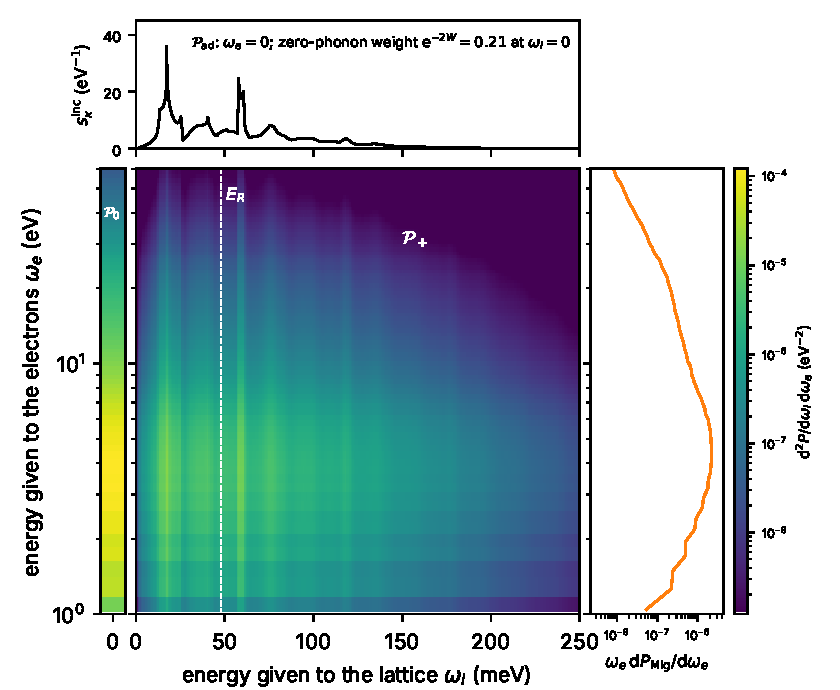
\includegraphics[width=0.92\linewidth]{figures/ch12/fig12_1.pdf}
  \caption{The joint response of silicon at $q = \SI{50}{keV}$ in the plane of the energy $\omega_l$ given to the lattice and the energy $\omega_e$ given to the electrons, per nucleus and normalized as probabilities, at $T = 0$. Top: the electron-following line $\omega_e = 0$, the incoherent lattice spectrum $s^{\mathrm{inc}}_\kappa$ of one nucleus without its zero-phonon part $\ee^{-2W} = 0.21$ at $\omega_l = 0$ ($E_R = \SI{47.8}{meV}$, $2W = 1.57$, phonon density of states from density-functional perturbation theory). Main panel: the Migdal probability density $\dd^2P/\dd\omega_l\,\dd\omega_e$ in the phonon-dressed sector $\mathcal{P}_+$; the dashed line marks $E_R$. Left strip: the zero-phonon Migdal line $\omega_l = 0$ (sector $\mathcal{P}_0$), drawn as a bin of \SI{1}{meV} in $\omega_l$ on the same color scale. Right: the marginal $\omega_e\,\dd P_{\mathrm{Mig}}/\dd\omega_e$. Model: \cref{eq:12.1-Skk} with valence electrons only, the ion charge $Z_{\mathrm{ion}}(p)$ of \cref{eq:12.3-Zion} and the diagonal $\vect{G} = \vect{G}'$. The electronic factor is the random-phase loss function of silicon with local fields of Knapen, Kozaczuk and Lin~\cite{knapen2021dark} (threshold \SI{1.11}{eV}, the step-model gap that accompanies the tables, $p \le \SI{22.5}{keV}$, $\omega_e \le \SI{89}{eV}$, averaged over directions); the transition densities are Condon in the frame of the crystal (lattice factor at $|\vect{q} - \vect{p}|$), and the lattice response is incoherent.}
  \label{fig:12-plane}
\end{figure}

The energy denominators of the boost neglect the nuclear motion against $\omega_e$, at relative order $v_Np/\omega_e$ and $(\omega_l/\omega_e)^2$; at the momenta of \cref{fig:12-plane} these are $3\times10^{-3}$ and $10^{-4}$. The exact denominators are \cref{eq:12.3-bracket} for a free nucleus and \cref{eq:12.4-exact} for a bound one. The Condon approximation drops the change of the transition density with the displacements, the Herzberg--Teller term above. The ground-surface final states drop the displacement of the excited surface, which moves energy from $\omega_e$ to $\omega_l$ without changing their sum, and which is negligible for a delocalized pair. \Cref{we:12-oscillator} shows the Herzberg--Teller term and the excited-surface displacement at work where they are not small.

\Cref{app:E.6} gives the dielectric matrix of the electrons, with local fields, on a grid of $(\vect{k}, \omega_e)$, and \cref{app:E.17} gives the lattice response on a grid of momenta.

\begin{workedexample}{The joint response of a displaced oscillator}\label{we:12-oscillator}
We take the model, the kick $\ee^{\ii qx}$ with $q\ell_0 = 1$ ($E_R = \omega_0 = \SI{64.1}{meV}$) and the labels of \cref{we:8-sectors}. A state on the excited surface with vibrational level $m$ gets $\omega_e = \SI{1.0463}{eV}$, the zero-phonon energy of the upper level, and $\omega_l = m \times \SI{65.5}{meV}$, the quanta of the excited surface, both read off the exact diagonalization.

\emph{The exact plane.} The line $\omega_e = 0$ carries the kick on the ground surface, with weight $1 - P_{\mathrm{Mig}}$. The Migdal weight $P_{\mathrm{Mig}} = 3.94\times10^{-6}$ of \cref{we:8-sectors} lies on the line $\omega_e = \SI{1.0463}{eV}$ as a comb in $\omega_l$, with the fractions 0.097, 0.227, 0.265, 0.205, 0.119 and 0.055 for $m = 0$ to 5. The lattice receives on average \SI{0.153}{eV} in a Migdal event, more than twice the recoil energy.

\emph{The leading entry with ground-surface final states.} This entry is \cref{eq:12.1-Skk}: every Migdal event sits at the vertical energy $\omega_e = \Delta_{\mathrm{tl}} = \SI{1.17}{eV}$, and the lattice factor is the kick of the ground surface, Poisson distributed with mean $(q\ell_0)^2 = 1$. The fractions are 0.368, 0.368, 0.184, 0.061, and the mean lattice energy is $E_R = \SI{64.1}{meV}$. The total energy per event, $\Delta_{\mathrm{tl}} + E_R = \SI{1.234}{eV}$, is close to the exact \SI{1.199}{eV}, but the split between electrons and lattice is wrong.

\emph{Excited-surface final states.} Projecting the kicked state on the vibrational states of the excited surface puts the relaxation energy in $\omega_l$. For surfaces of equal frequency the overlap $\langle m_{\mathrm{up}}|\ee^{\ii qx}|0_{\mathrm{lo}}\rangle$ is that of a coherent state whose amplitude adds the imaginary kick $\ii q\ell_0$ to the real displacement $-S_{\mathrm{HR}}^{1/2}$. The weights are then Poisson with mean $(q\ell_0)^2 + S_{\mathrm{HR}} = 3$, and the mean lattice energy is $3\omega_0 = \SI{0.192}{eV}$, against $E_R$ before. On the computed surfaces, with their unequal quanta, the same projection gives the mean lattice energy \SI{0.188}{eV} and the zero-phonon fraction 0.056 instead of $\ee^{-3} = 0.050$, with the derivative coupling evaluated at $x = 0$ (the Condon approximation). The relaxation energy $S_{\mathrm{HR}}\omega_0 = \SI{0.128}{eV}$ has moved from $\omega_e$ to $\omega_l$, and the total $\SI{1.0463}{eV} + \SI{0.188}{eV} = \SI{1.234}{eV}$ is unchanged. The probability is $3.52\times10^{-6}$, the value of the boost formula of \cref{we:8-sectors}, and the zero-phonon fraction 0.056 falls short of the exact 0.097.

\emph{Beyond Condon.} The derivative coupling and the gap both vary along $x$: the gap is $\Delta_{\mathrm{tl}} + g_{\mathrm{d}}x/\ell_0$, smaller on the side of the displaced minimum. Keeping $q\,d_{10}(x)/[(M/2)\Delta E(x)]$ inside the vibrational matrix element, as a function of $x$, gives $P_{\mathrm{Mig}} = 4.00\times10^{-6}$, the fractions 0.104, 0.236, 0.267, 0.201, 0.113 and 0.051, and the mean lattice energy \SI{0.148}{eV}, all within a few percent of the exact values. \Cref{we:8-sectors} traced the \SI{12}{\percent} excess of the exact probability over the boost formula to the displaced surface; this excess is the Herzberg--Teller term, and it acts most on the zero-phonon line.

A strongly displaced excited surface, as for an exciton bound to a defect, therefore needs the zero-phonon energy as its electronic energy and the non-Condon term. For an electron--hole pair spread over $N$ cells, $S_{\mathrm{HR}}$ is of order $1/N$, and the ground-surface form \cref{eq:12.1-Skk} is the right one.
\end{workedexample}

\subsection{Local fields and the choice of electrons}\label{sec:12.1-truncations}

Each truncation of \cref{fig:12-map} keeps the boost and makes a choice for the vertex, the electronic factor and the lattice factor. On the diagonal of $\varepsilon^{-1}$ the local fields lower the silicon probability by a factor 1.35 against a scalar dielectric function (\cref{lim:12.3a}). Through the off-diagonal elements $\vect{G} \neq \vect{G}'$ they couple different momenta. No table in this book contains the off-diagonal part; it is sized only in a model of silicon, where it raises the rate, and the full calculation is still open (\cref{sec:12.3-validity}). The same matrix $\varepsilon^{-1}$ changes the electron-recoil rate of silicon by a factor of 1.5 at \SI{10}{MeV} (\cref{sec:10.2-corrections}). The atomic formula, applied to the valence electrons of a crystal, puts the wrong electrons in the electronic factor. The valence electrons of silicon are not those of a silicon atom, and their gap is \SI{1.17}{eV} instead of the atomic binding of several eV; the factor $\omega_e^{-4}$ magnifies the difference between the two energies. For the core shells, whose electrons do move with their nucleus, the atomic form is the right truncation (\cref{sec:12.2}).

\subsection{Double counting of recoils}\label{sec:12.1-counting}

The joint response holds the lattice and the Migdal parts of one nuclear response, and its moments fix how they add. Take the incoherent response, one nucleus at a time. The total weight of $n_\kappa(\vect{q})$ is $2\pi\nd_\kappa$, the density of nuclei times $2\pi$, whatever the final states; integrated over the plane, \cref{eq:12.1-joint} has that weight. The Migdal entry takes $2\pi\nd_\kappa P_{\mathrm{Mig}}(q)$ of it, and the line $\omega_e = 0$ keeps
\begin{equation}
  \int\dd\omega_l\;S^{\mathrm{ad}}_{\kappa\kappa}(\vect{q},\omega_l) = 2\pi\nd_\kappa\bigl[1 - P_{\mathrm{Mig}}(q)\bigr] .
  \label{eq:12.1-zeroth}
\end{equation}
The first moment of the line, by \cref{eq:8.6-fsum-k}, is that of a nucleus of mass $M_\kappa + \delta M_\kappa$. The lattice responses of \cref{chap:11} are normalized to unit weight and use the bare mass. Added to a Migdal rate, they count twice the kicks that excited the electrons: once as pure recoils on the line $\omega_e = 0$ and once as Migdal events. The double count is a fraction $P_{\mathrm{Mig}}$ of the kicks, but in each of them the lattice energy is not small: \cref{fig:12-plane} shows that a Migdal event carries the whole recoil, \SI{48.5}{meV} on average against $E_R = \SI{47.8}{meV}$, and the electronic energy on top of it. The consistent sum takes the lattice response with the weight $1 - P_{\mathrm{Mig}}$ and the mass $M_\kappa + \delta M_\kappa$, the first prescription of \cref{sec:8.6}, and the joint response applies this prescription by construction. In silicon the weight correction $P_{\mathrm{Mig}}$ and the mass correction $\delta M_\kappa/M_\kappa$ are both below $10^{-3}$ for $E_R \lesssim \SI{16}{eV}$, which covers the phonon and multiphonon momenta of \cref{chap:11}, and the rate of a phonon detector does not see the two corrections there. At \SI{500}{eV} the weight $1 - P_{\mathrm{Mig}}$ is a \SI{3}{\percent} correction (\cref{sec:12.5-bounds}). The counting of Migdal and lattice events, however, is exact, and \cref{sec:12.5} completes it with the higher moments.

The same entry fixes the lattice factor of the Migdal rate itself. A Migdal event leaves the lattice in the state that the kick $\vect{q} - \vect{p}$ makes, so the lattice factor of a Migdal rate below the impulse onset is the multiphonon response of \cref{sec:11.3}, not a free recoil. Combining a free-recoil Migdal formula with a multiphonon lattice rate counts nothing twice; it mixes two truncations of one response, and a rate built that way is labeled by neither. On the scale of \cref{sec:8.5} the two pieces of a rate should carry the same lattice regime $\mathcal{K}$.

Measured nuclear-recoil signals obey the same rule from the other side. A calibration with neutrons measures the ionization of nuclear recoils, and the Migdal electrons of those recoils are part of what it measures. A nuclear-recoil rate converted to charge with a measured yield already contains the Migdal ionization, and a computed Migdal rate added to it counts that ionization twice. The yield and its Migdal part are separated in \cref{sec:19.2}.

\subsection{Targets without a gap}\label{sec:12.1-gapless}

The construction used the gap three times: to give each final state an electronic energy, to make the energy denominators of the boost large compared with the lattice energies, and to keep the low-energy end of $S^{ee}$ empty. In a metal, a superconductor or a semimetal all three fail.

With the quasiparticle sectors $\mathcal{P}^{\mathrm{qp}}_{n,m}$ of \cref{sec:8.6}, $\omega_e$ becomes the energy of the quasiparticles created, defined to within their width, and the joint response is meaningful on bins of the plane that satisfy the bin bound \cref{eq:8.6-bin}.

In a metal the loss function grows linearly from $\omega_e = 0$, since electron--hole pairs at the Fermi surface cost nothing, and with the factor $\omega_e^{-4}$ the Migdal probability \cref{eq:12.1-Skk} integrates as $\int\dd\omega_e\,\omega_e^{-3}$ and diverges at small $\omega_e$. The divergence marks the failure of the sudden expansion, not a large effect. Once $\omega_e$ falls to the phonon energies, the electrons follow the nucleus instead of being left behind. The boost denominator $\omega_e^2$ must then be replaced by the full denominator. For a bound nucleus the full denominator is the phonon propagator $\omega_e^2 - \omega_{\mathrm{ph}}^2$ of the phonon-mediated form, whose pole at $\omega_e = \omega_{\mathrm{ph}}$ is the ordinary electron--phonon coupling of \cref{chap:6}. The part of the plane with $\omega_e \lesssim \omega_{\mathrm{D}}$ then belongs to the electron--phonon response of the metal, computed with Fan--Migdal and Eliashberg methods (\cref{sec:6.3,sec:6.4}), and only $\omega_e \gg \omega_{\mathrm{D}}$ is a Migdal process in the sense of this chapter. The electronic factor also changes character: $S^{ee}$ contains the intraband response of the conduction electrons, which screens the moving ion at small $\omega_e$, so that a slowly moving ion in a metal carries no charge. The full response contains this intraband screening, and a formula that screens the vertex statically does not. In a superconductor, whose hierarchy is reversed (\cref{sec:8.6}), a kicked nucleus breaks pairs through the phonons it emits (\cref{chap:15,chap:20}).
